\section{Ozone}

Ozone absorbs in the solar wave length spectrum but also in the
thermal wave length spectrum thus acting as a greenhouse
gas. According to \citet[p.528]{brasseur1999} 
it contributes about 16\% to the total radiative forcing due to
increases in greenhouse 
gas concentrations for the period from 1900 to 1990.
The mass mixing ratio of ozone in the
atmosphere strongly varies with altitude and geographical
latitude. The variation with geographical longitude at fixed latitude
and altitude are less pronounced but not negligible. Therefore, it is
preferable to use 3--dimensional ozone data. The ozone concentration
also depends on time, but climatological data may be useful for
non--transient simulations.
 
\subsection{Historic}

The data set for historic ozone concentrations was created within the projects
AC\&C and SPARC for simulations (e.g.~CMIP5)
that do not take interactive chemistry into account
(\cite{cio117}). The ozone data 
are prepared using
satellite (SAGE~I and~II) and radiosonde data for the stratosphere
and model data (CAM3.5 and NASA-GISS PUCCINI) for the troposphere.
These historic ozone data include the ozone reduction in the
stratosphere caused by ozone depleting species.
A short description of the construction is given on:
\newline
{\tt http://www.pa.op.dlr.de/CCMVal/AC\&CSPARC\_O3Database\_CMIP5.html.}\newline

Ozone data are provided in terms of 3--dimensional monthly
averages. However, in the stratosphere 
the data set does not vary with longitude, so that only in the troposphere
real 3D information is available.

Original data exist only for altitudes with
pressures larger than 1~hPa. Since the standard vertical resolutions
include model layers with pressures as low as 0.01~hPa, 
the dataset was extended upward by
Chris Bell (University of Reading) applying the following
formula:\\
\begin{equation}
O_3(z) = O_3(1~\textrm{hPa}) * \exp(-(z-z(1~\textrm{hPa}))/H),
\end{equation}
with $H$ set to 7 km and $O_3(z)$ denoting the ozone concentration at altitude $z$. 

The resulting 3--dimensional ozone data for the years 1850--2008 are given as
monthly mean values on 39~pressure levels which are listed in
Table~\ref{tabpres}. The data are organized in yearly files {\tt
  T\{RES\}\_ozone\_CMIP5\_{\it yyyy}.nc} where {\tt \{RES\}}
represents the horizontal resolution and {\tt\it yyyy} the
respective year between 1850 and~2008. These files contain the
pressure levels in the variable {\tt plev} and the ozone volume mixing
ratio in the variable {\tt O3}. Height interpolation is performed by \echam. 

\begin{table}[hb]
\caption{Pressure levels in~Pa of ozone climatology}\label{tabpres}
\begin{tabular*}{\textwidth}{c@{\extracolsep\fill}ccccccc}\hline
\cw{00000}1& \cw{00000}3& \cw{00000}5& \cw{0000}10& \cw{0000}20&
\cw{0000}30& \cw{0000}50& \cw{000}100 \\
\cw{000}150& \cw{000}200& \cw{000}300& \cw{000}500& \cw{000}700&
\cw{00}1000& \cw{00}1500& \cw{00}2000 \\ 
\cw{00}3000& \cw{00}5000& \cw{00}7000& \cw{00}8000& \cw{0}10000&
\cw{0}15000& \cw{0}20000& \cw{0}25000 \\ 
\cw{0}30000& \cw{0}40000& \cw{0}50000& \cw{0}60000& \cw{0}70000&
\cw{0}85000& 100000 & \\\hline 
\end{tabular*}
\end{table}

\subsection{Scenarios}
Future ozone scenarios for the period 2008--2099 are provided from the
same source mentioned in the case of historic data. 
In the case of the future the data set is based on multi--model
projections provided in the  
framewok of the SPARC Chemistry-Climate Model Validation Activity
(CCMVAL, see \cite{cio117,eyr103}).
As in the case of historical ozone the original dataset also did only
extend up to 1 hPa 
and was extended upward by Chris Bell. This dataset however does not
include a solar cycle. 
For CMIP5 simulations with \echam
solar cycle 23 is repeated for the future, i.e. the solar variability for
the period May 1996 to July 2008 is repeated for August 2008 to
October 2020, November 2020 to January 2033, etc. (see
section~\ref{sec:externaldata_solar}). 
In order to obtain future ozone concentrations consistent with the
assumptions for solar irradiance 
a multi-linear regression analysis was performed for the historical
ozone data using  the solar irradiance 
at a wavelength of 180.5 nm and the EESC (Equivalent Effective Stratospheric Chlorine) content as regressors.
The resulting regression coefficients for the ozone dependence on solar irradiance and the assumed future irradiance at 180.5 nm 
were then used to add a solar cycle dependence to the future
stratospheric ozone. Tropospheric data (for $p \ge 100$ hPa) have not
been 
modified as the solar cycle dependence calculated from the historic
data for this altitude regime is negligible.  

AC\&C/SPARC ozone projections are available only until 2099. For the
years starting with 2100 the 
original ozone data for the year 2099 are used, but modulated by a
solar cycle effect as described above for the years 
until 2099. Data files were prepared until the year 2399.

The total column ozone for various geographical regions for the
years 1850 to 2099 is presented in Fig.~\ref{fig:ozone}.

\begin{figure}[htb]
\[
\ifpdf
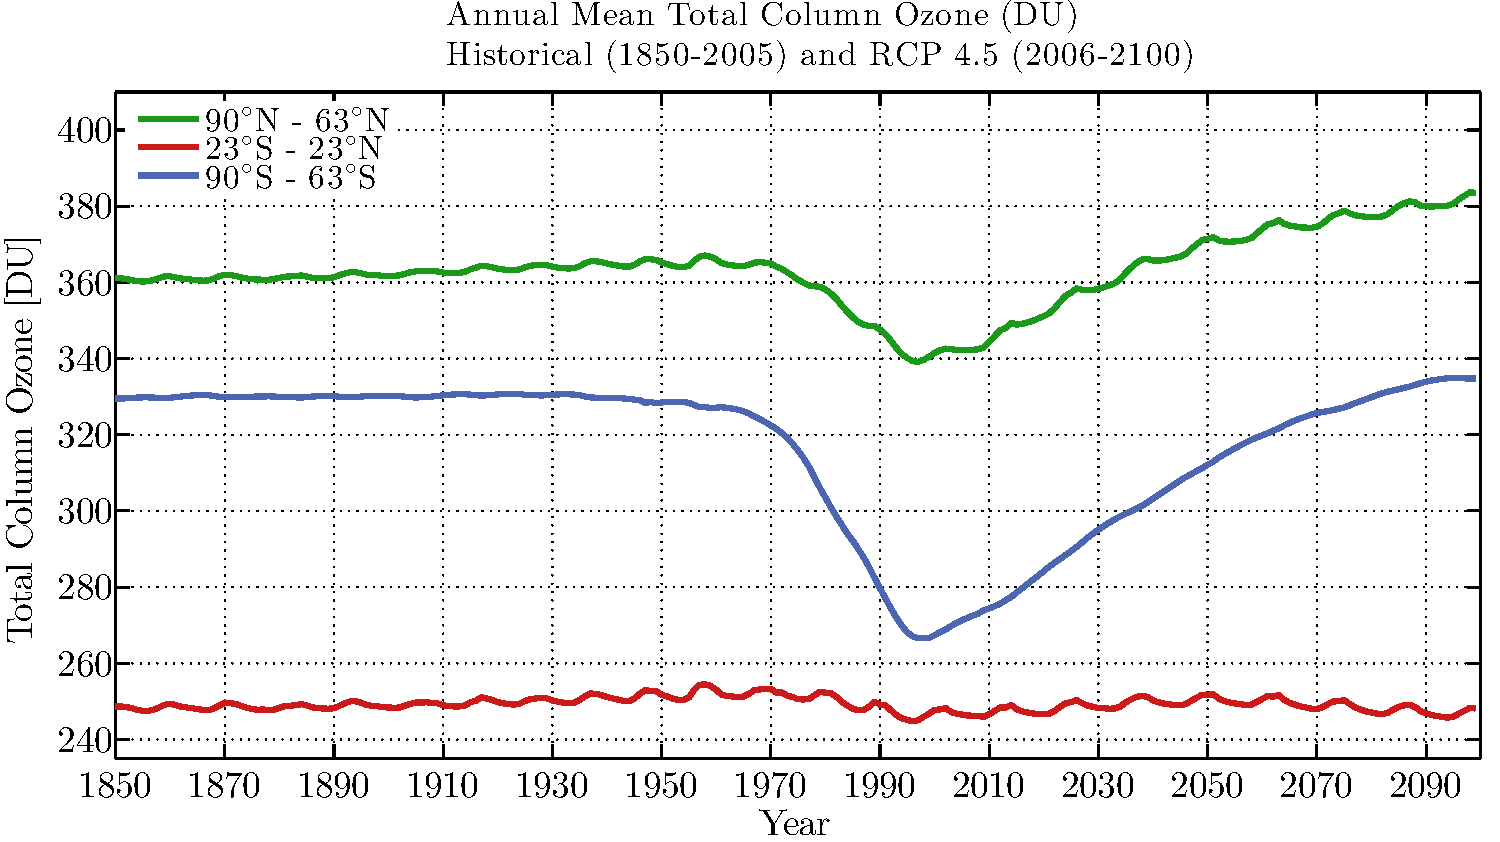
\includegraphics[width=12cm]{externaldata/total_column_ozone_annual.pdf}
\else
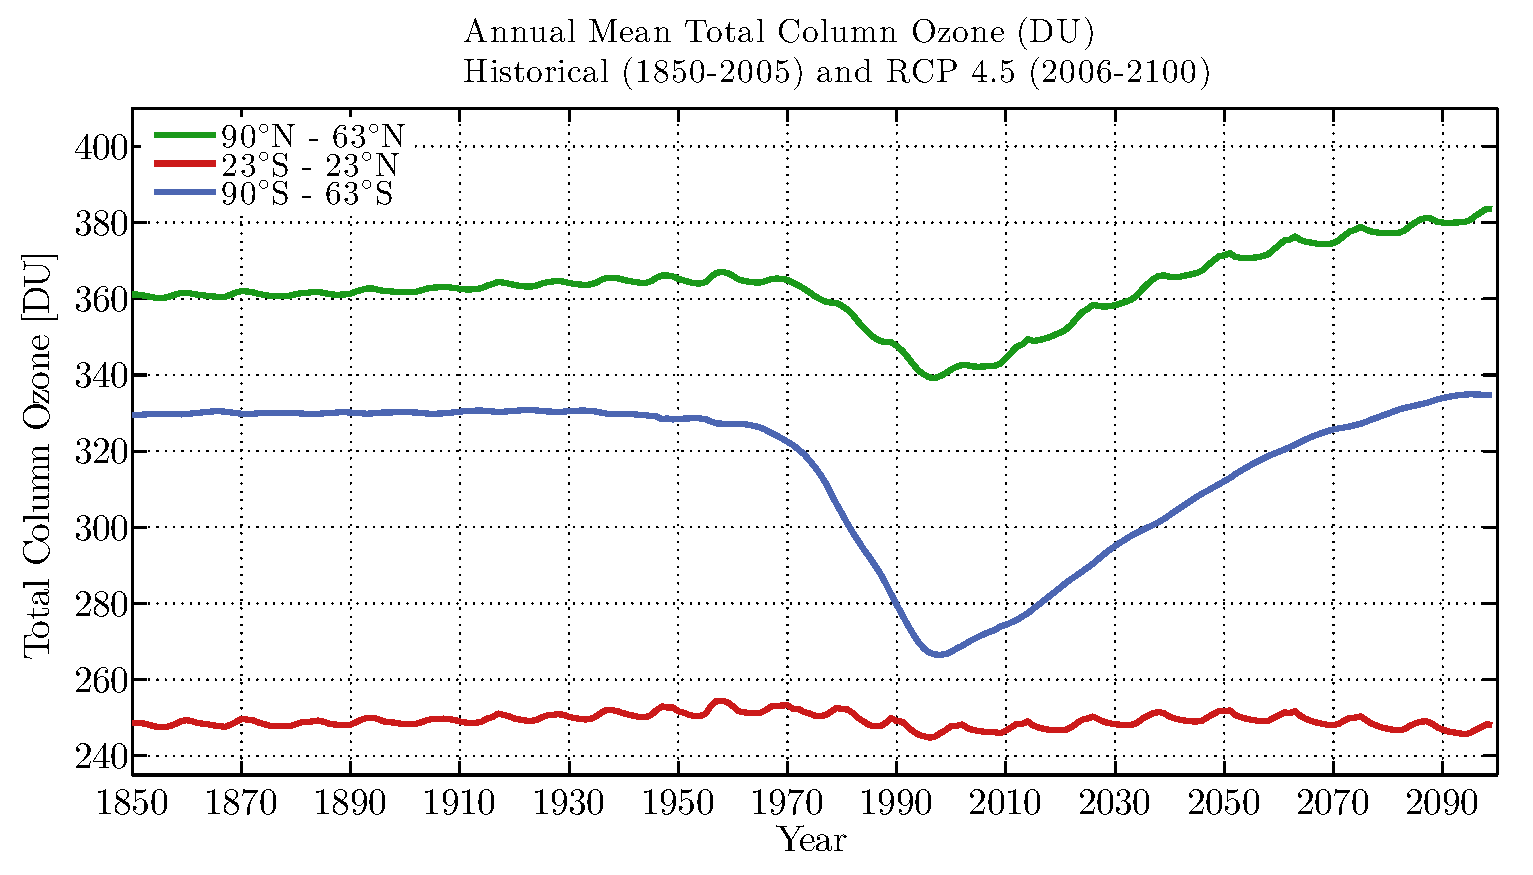
\includegraphics[width=12cm]{externaldata/total_column_ozone_annual.eps}
\fi
\]
\caption{Annual total column ozone for various geographical regions
  for the years 1850 to 2099. Figure courtesy by Alexander Haumann}\label{fig:ozone}
\end{figure}


As in the case of historical data, 3--dimensional ozone data for the
years 2009--2399 are given as 
monthly mean values on 39~pressure levels.
The data are organized in yearly files 
{\tt T\{RES\}\_ozone\_CMIP5\_\{rcp\}\_{\it yyyy}.nc} where {\tt \{RES\}}
represents the horizontal resolution and {\tt\it yyyy} the
respective year. \{rcp\} can have the values RCP26, RCP45 or RCP85,
and indicates the respective representative concentration pathway   
(i.e. future greenhouse gas scenario) for which the data set is valid. 
While in the stratosphere (for $p < 100$ hPa) all data sets are equal,
the AC\&C/SPARC projections differ for tropospheric ozone. 





\subsection{Climatologies}

In some cases, mean values of historic ozone concentration over time
may be used as climatological boundary condition. Therefore, monthly
mean ozone 
concentrations over eleven years for the years 1850--1860 ({\tt
  T\{RES\}\_ozone\_CMIP5\_1850-1860.nc} to be used for preindustrial simulations
  and the years 1979-1988 ({\tt
  T\{RES\}\_ozone\_CMIP5\_1979-1988.nc}) are also provided. In both cases the averaging
was performed over about one full solar cycle in order to avoid potential
biasing from biased solar irradiance.
